\Chapter{Megvalósítás}

Ebben a fejezetben kerül részletes bemutatásra a program implementációjának folyamata, kiegészítve a nehézségekkel, problémákkal és azok megoldásával. 

Mivel a csomagadatok lekérdezése egyszerűen megoldható az npm Registrynek köszönhetően, így gond nélkül lehet keresést implementálni, amelynek eredményeként megkaphatjuk egy adott csomag adott verziójának összes függőségét.

\section{Csomag Szerkezet}
Az npm csomagok szerkezetére vannak megkötések, így a projekt szerkezetét is ilyen formára kell hozni. Elkészült hozzá a \texttt{package.json} fájl, amely tartalmaz minden kötelező és releváns opcionális mezőt. A csomag a \textbf{package-examiner} fantázianevet kapta.   

A csomag belépési pontja, a \texttt{package.json}-ban is jelzett \texttt{main.js}. A csomag funkcionális szerkezete az alábbi módon néz ki:

\begin{js}
./	
	src/
		- scripts
		- styles
		- templates
		- app.js
		- main.js
	public/
		- index.html
	package.json
	package-lock.json
	README.md	
\end{js}

Mint látható csak az \texttt{index} HTML fájl létezik, ennek oka a következő szakaszban részletezésre kerül.

\pagebreak

\section{Single-Page UI}

A Single Page Application, azaz SPA lényege, hogy egy oldalra dinamikusan tölti be a tartalmat, nem történik új lap nyitása, se újratöltés.

Ennek a megvalósítására több technológia létezik, többek között a jQuery könyvtár is. A program úgynevezett "JavaScript Template"-ekkel való megoldást alkalmazza, amely során JavaScript fájlokban hoz létre HTML sablonokat és azokat exportálja, majd az applikáció felhasználási módtól függően dinamikusan tölti be azokat.\\

\textbf{Egy ilyen exportálható JavaScript Template szintaktikája:}

\begin{js}
	const Template = () => {
		const template = `
		#Some HTML code
		`;
		return template;
	};

	export default Template;
\end{js}

A program az alábbi sablonokat tartalmazza:
\begin{js}
./templates/	
	Sidebar
	- Examiner.js
	- Statistics.js
	Canvas.js
	Sidebar.js
\end{js}

A Sidebar és Canvas sablonokat az app.js fájl tölti be automatikusan az index.html-be, ezek konstansan részét képezik az index tartalmának. A Sidebar és a Canvas tartalmának egy része azonban felhasználási módtól függően változik.

Az Examiner-t egy csomag, a Statistics-t több csomag vizsgálata estén tölti be. A két funkcionalitási mód közötti váltást egy "Switch Mode" gomb teszi lehetővé.\\

\begin{figure}[!h]
	\centering
	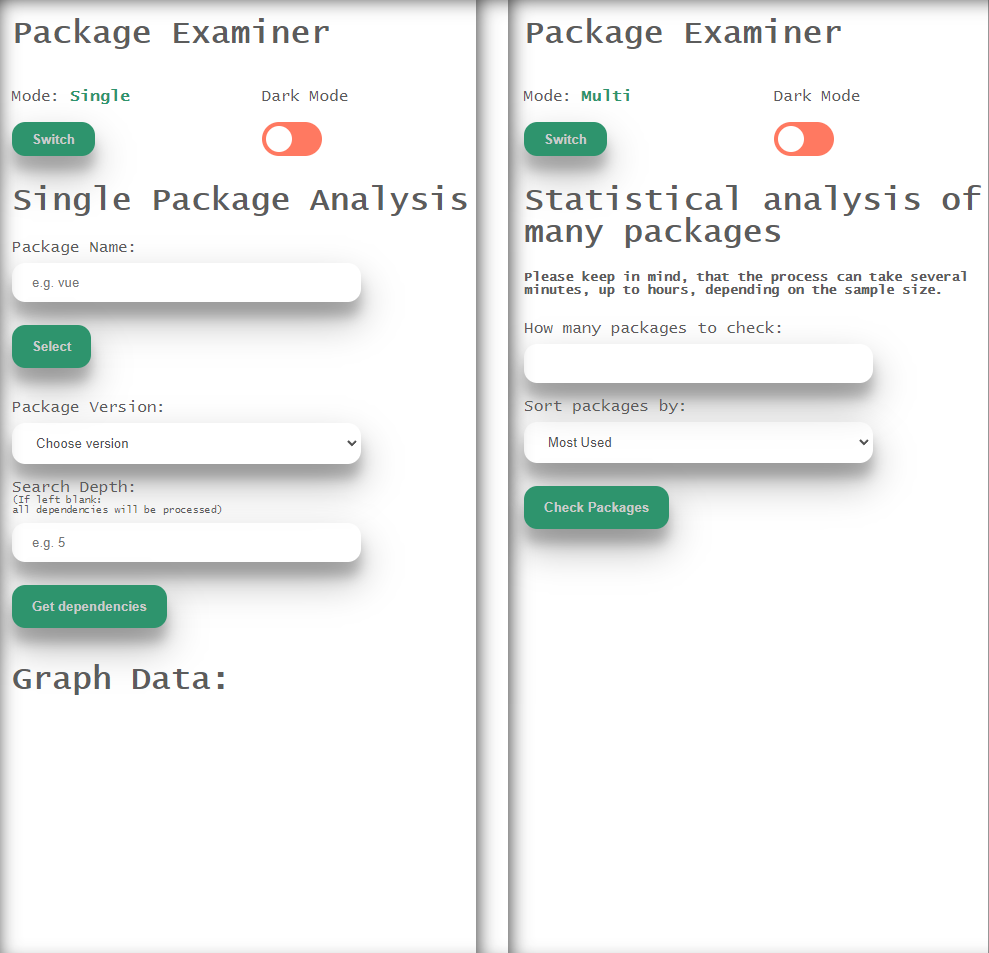
\includegraphics[scale=0.2]{images/ui_modes.png}
	\caption{Single / Multi Package Sidebar}
	\label{fig:ui_modes}
\end{figure}

\pagebreak


A \textbf{Single Package Analysis} esetén, ha létező csomagra keresünk rá, akkor automatikusan felölti a Package Version listát. Mivel a Registry-ben szükséges verziók szerint keresni, ez biztosítja a keresés sikerességét.\\

Amennyiben a Registry-ben csak a csomagnévre keresünk rá, akkor nem fogunk függőségeket visszakapni, mivel itt általános információk vannak a csomagról, nem pedig működési információk. Konkrét információt a verzió megadásával tudunk megszerezni.\\

A Sidebar továbbá tartalmaz egy konstansan jelen lévő kapcsolót, amellyel a világos és sötét megjelenítési mód között lehet választani, az alapértelmezett mód a sötét, viszont \underline{nyomtatási szempontból} a \textbf{világos módot} fogom használni az ábrákhoz. 

\begin{figure}[!h]
	\centering
	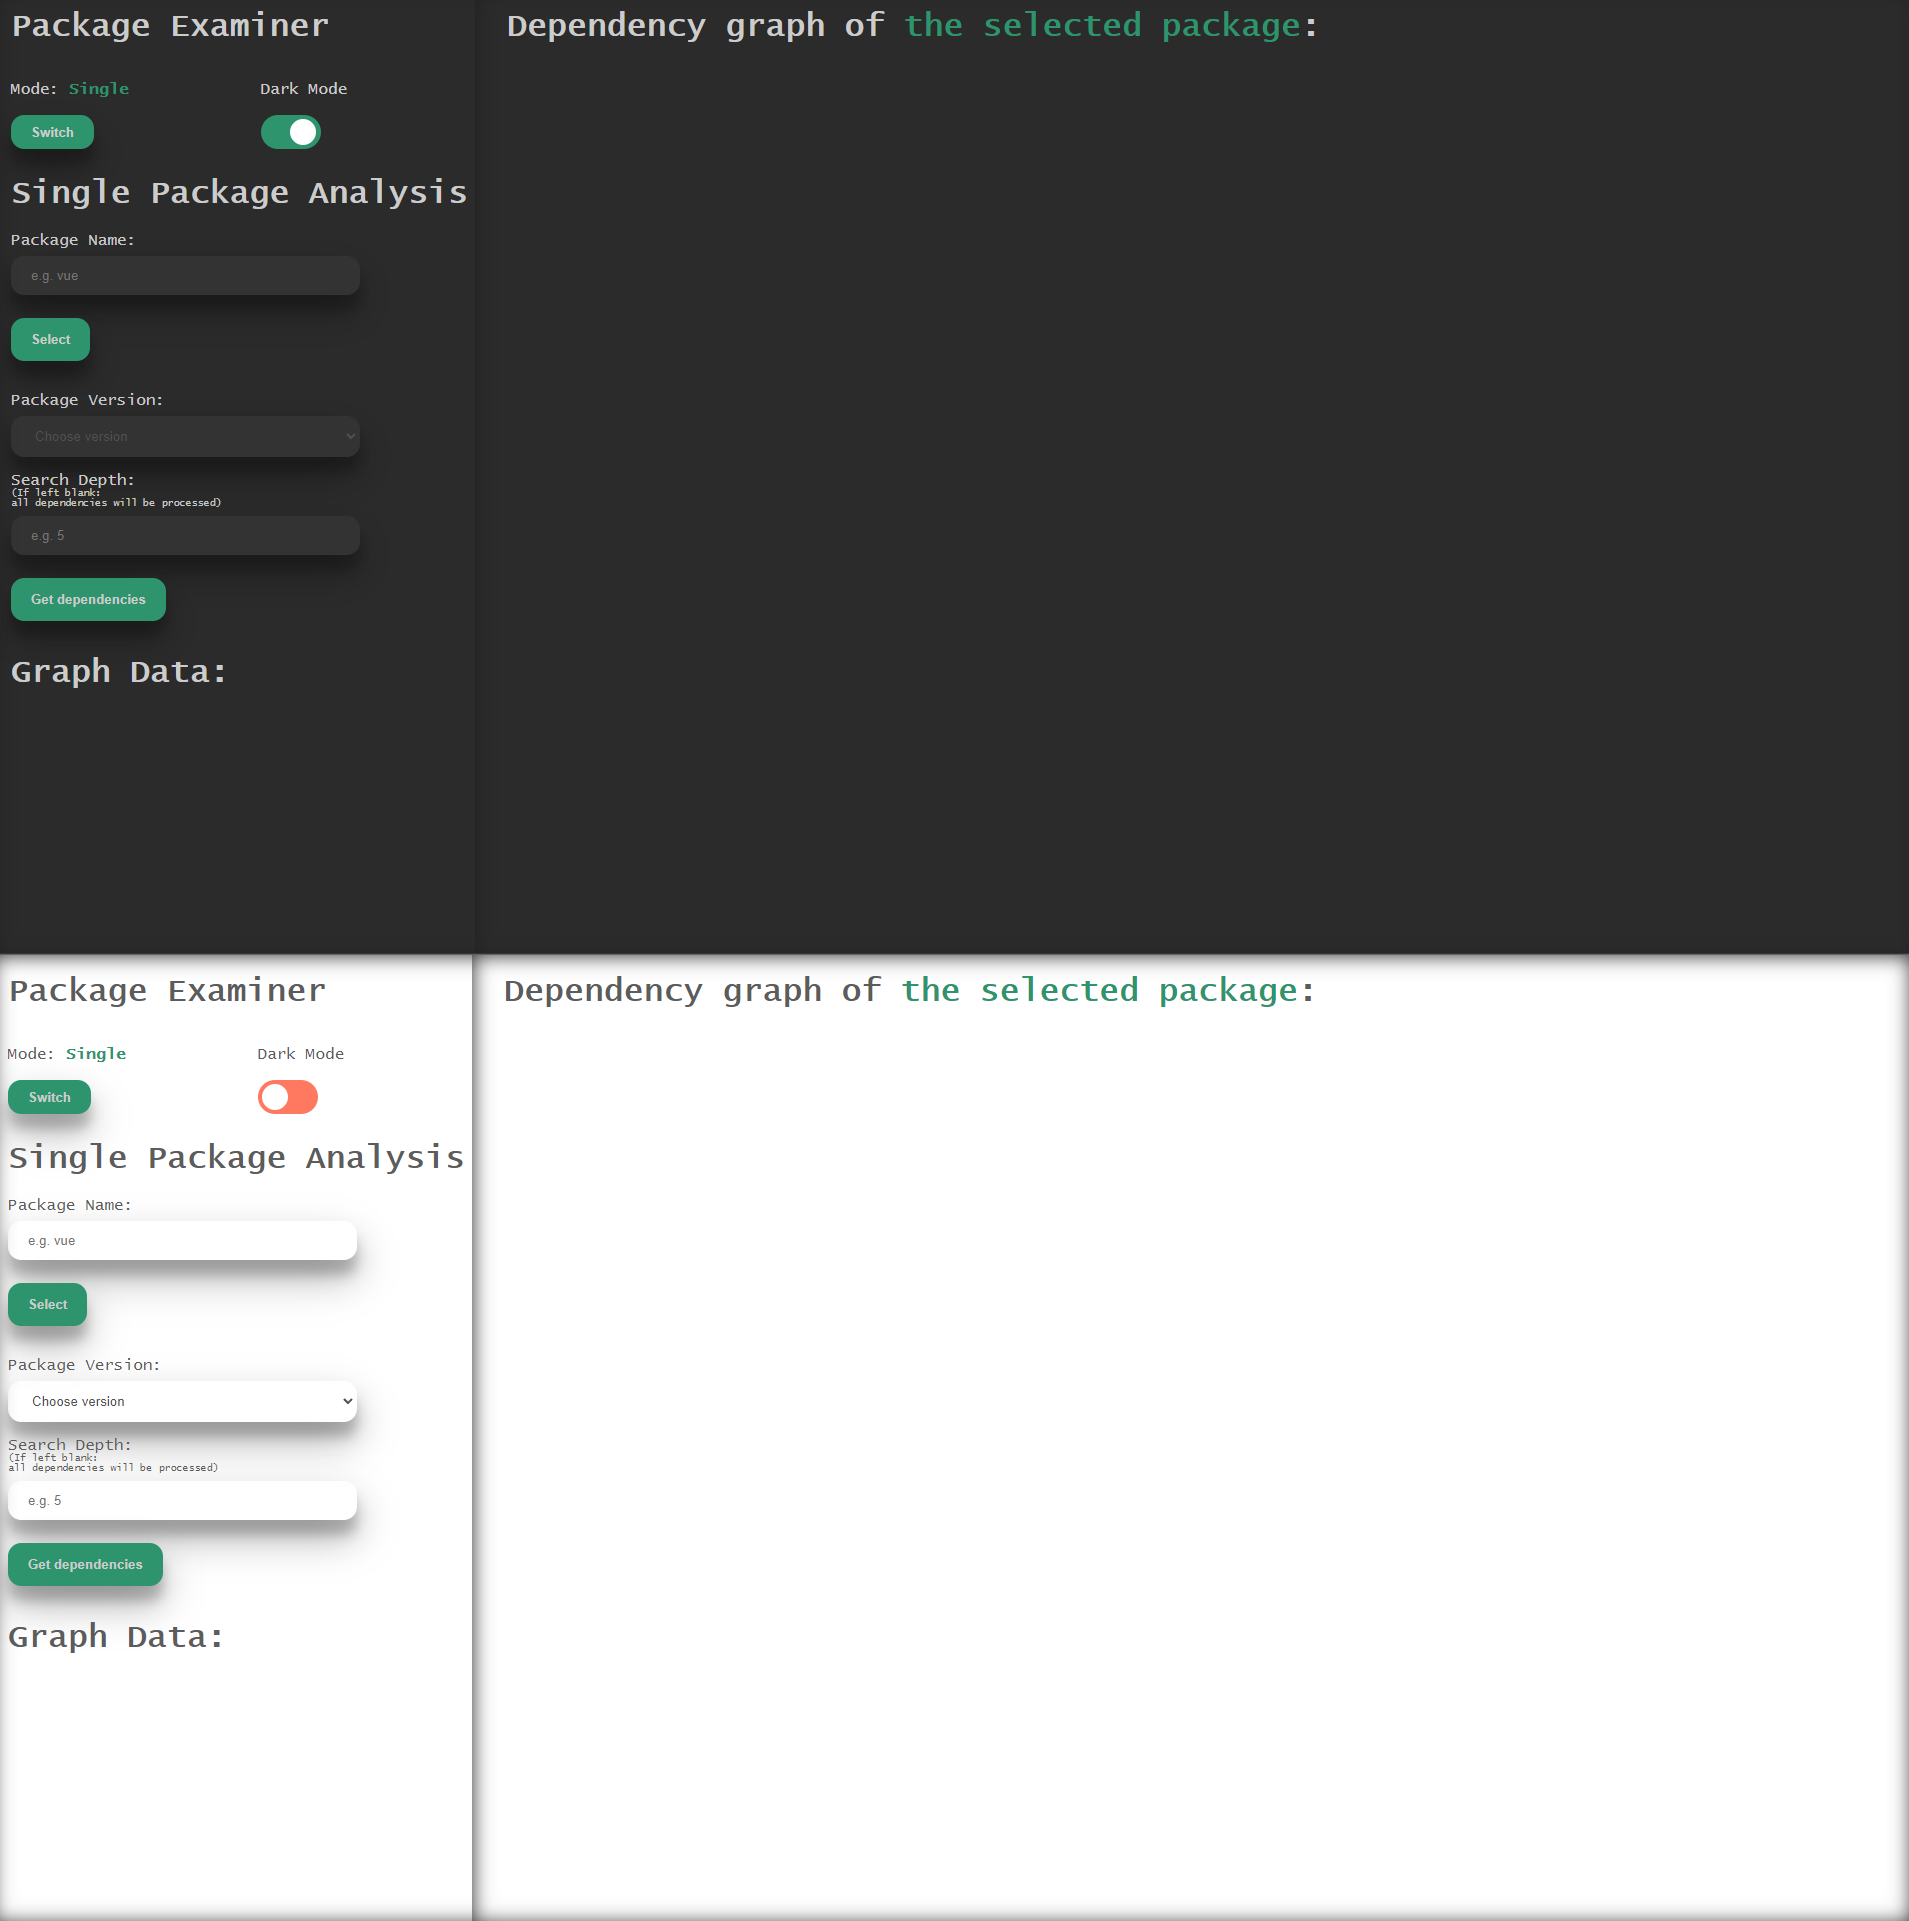
\includegraphics[scale=0.15]{images/ui_darkmode.png}
	\caption{UI Sötét/Világos mód}
	\label{fig:ui_darkmode}
\end{figure}

A csomagok adatainak lekérdezését, függőségek összegyűjtését, elemzését és ábrázolását végző funkciókat a következő "lekezelő" funkció indítja el, amint a szükséges információk ki vannak gyűjtve:

\begin{js}
window.handleFormEvents = (event) => {
	event.preventDefault();
	submitForm(event.target.id);
};
\end{js}

\pagebreak

\section{Adatgyűjtés}

Az adatok lekérésére három különböző modul áll rendelkezésre, a \textbf{getPackage.js}, a \textbf{searchPackages.js} és a \textbf{getGitData.js}.

A program HTML form-ok küldés eseményére reagál, majd ezeket lekezeli és a form típusától függően hív meg függvényeket. Ezt a \textbf{handleSideBarEvents.js} modul fogja végezni, mely az alábbiak szerint dönti el, hogy mely funkciókat hívja meg:

\begin{js}
function submitForm(form){
	switch (form) {
		case "packageForm":
		getPackageData();
		break;
		case "graphingForm":
		makeGraph();
		break;
		case "statForm":
		makeStat();
		break;
		default:
		break;
	}
}
\end{js}

\noindent\textbf{getPackageData()}
\begin{itemize}
	\item Ez a funkció felelős a "Package Version" Select DOM elem listájának feltöltéséért. 
	\item Amennyiben nem található a csomag, hibát fog dobni.
	\item Közvetlenül támaszkodik a \textbf{getPackage.js} modulra.
\end{itemize}

\noindent\textbf{makeGraph()}
\begin{itemize}
	\item Ez a funkció felelős a kiválasztott csomag függőségei gráfjának megalkotásáért, megrajzolásáért, majd pedig elemzéséért.
	\item Amennyiben nincs kiválasztva a verzió, hibát fog dobni.
	\item Közvetetten támaszkodik a \textbf{getPackage.js} modulra.
\end{itemize}

\noindent\textbf{makeStat()}
\begin{itemize}
	\item Ez a funkció felelős több csomagos mód esetén a megadott paraméterek szerinti csomagok összegyűjtéséért, függőségi elemzéséért és statisztikai ábrázolásáért.
	\item Amennyiben nem található a csomag, hibát fog dobni.
	\item Közvetetten támaszkodik a \textbf{searchPackages.js} és \textbf{getGitData.js} modulokra.
\end{itemize}

\pagebreak

\subsection{Lekérdezések}

\textbf{Probléma:} Az npm Registry lekérdezésénél lehetőség van egy csomag adatainak lekérésére, illetve arra is, hogy a Registry-ben található csomagok között keressünk. Ezzel csak az a probléma, hogy a keresés a keresés szövege köré épül, tehát lényegében nem tudunk minden csomag esetében, megadott paraméterek szerint keresni, mivel legalább egy betűt elvár a keresési végpont.

\textbf{Megoldás:} A Libraries.io API-ja, amely lehetőséget ad arra, hogy popularitás, illetve egyéb szempontok szerint keressünk tetszőleges mennyiségű csomagot. Ez a több csomagos módnál szükséges lesz.

Az applikáció minden lekérdezése aszinkron, hogy ne befolyásolja a végfelhasználói élményt, így ameddig nincsenek adatok, törekedve arra, hogy a felhasználó tisztában legyen azzal, hogy a háttérben futnak a folyamatok, a képernyőn megjelenik egy körkörös, töltést jelző ikon.\\

\noindent 1) \underline{getPackage()}\\

\begin{js}
function getPackage(packageName, packageVersion="", requiredData=""){
	*do stuff*
	return pkg;
}
\end{js}

Ez a funkció egy csomagnevet vár el, illetve opcionálisan megadható a csomagverzió és arra is van lehetőség, hogy megadjuk, hogy a válaszként kapott objektumból milyen adatra van szükségünk.

A visszatérési érték a megadott paramétereknek megfelelő objektum lesz.

\noindent 2) \underline{searchPackages()}\\

\begin{js}
function searchPackages(size, sortBy){
	*do stuff*
	return pkgs;
}
\end{js}

Ez a funkció a lekérdezendő csomagok számát várja el, illetve, hogy mi alapján állítsa sorrendbe és adja vissza a tárolt adatokat.

A visszatérési érték a megadott paramétereknek megfelelő csomagokat tartalmazó objektum lesz.

\pagebreak

\subsection{HTTP Kérés}

A programon belül a HTTP kérések a fetch API segítségével valósulnak meg, amely a következő módon működik:

\begin{js}
async function fetchData(url){
	let response = await fetch(url);
	
	if (!response.ok) {
		throw new Error(response.status);
	}
	
	return response.json();
}
\end{js}

\textbf{async/await} módon működik, ígéretet ad arra, hogy fog adni adatot a meghívója számára, amely addig vár a futásával, de közben más feladatok futását nem akadályozza.

\textbf{URL:} Az URL attól függően, hogy egy csomag információira vagyunk kíváncsiak, vagy csomagokra bizonyos paraméterek szerint, a következő lehet:
\begin{itemize}
	\item Egy csomag esete: npm Registry (https://registry.npmjs.cf/)
	\item Több csomag esete: Libraries.io (https://libraries.io/api/search)
\end{itemize} 

\section{Gráfalkotás és Elemzés}

A \textbf{makeGraph()} funkció meghívásával kezdődik el a folyamat. A függvény amennyiben ki van választva egy csomag és annak egy verziója, meghívja a \textbf {grahpDependencies.js} modult. 

\begin{js}
function graphDependencies(pckg, dDepth, singleMode=true){
	
	let dependencies = await getDependenciesTillDepth(pckg, dDepth);
	let packages = dependencies[dependencies.length-1];
	dependencies.pop(dependencies[dependencies.length-1]);
	
	let graphEntities = 
		calculateGraphData(packages, dependencies, singleMode);
	let currentGraph = 
		new Graph(graphEntities[0], graphEntities[1]);
	
	if(singleMode){
		analyseGraph(currentGraph);
	}
	
	return currentGraph;
}	
\end{js}

Egy és több csomagos módban is a makeGraph() a kiindulópont, mivel ez a funkció felelős egy adott csomag függőségeinek összegyűjtéséért, azok gráf struktúrába rendezéséért.
Visszatérési értékként a csomag függőségi gráf struktúráját adja vissza.\\

A \textbf{singleMode} boolean jellegű változó 'igaz' (alapértelmezett) érték esetén a következő extra funkciók is végrehajtásra kerülnek:
	\begin{itemize}
		\item A gráf struktúra kirajzolása
		\item A gráf analizálása
	\end{itemize}

Következő lépésként fog megtörténni az adott csomag függőségeinek megkeresése. Ezt a \textbf{getDependencies.js} modul fogja teljesíteni, amely az alábbi 3 függvényt tartalmazza:

\begin{js}
function getDependenciesTillDepth(pckg, depth){
	*do stuff*
	return dependencies;
}

function populateDependencies(pckg, depth){
	*do stuff*
	return dependencies;
}

function getDependencies(pckg){
	*do stuff*
	return returnDeps;
}
\end{js}

\subsection{A getDependencies modul}

Először a \textbf{getDependenciesTillDepth()} függvény kerül meghívásra, ez attól függően, hogy megadták-e hogy milyen mélyen keressen fogja megkeresni az adott csomag függőségeit, majd ezeket egy tömbként fogja visszaadni. A tömb utolsó elemét mindig a csomagok tömbje képzi, amelyektől függ a kiinduló csomag.\\

\textbf{Mélység: }A keresés mélysége az a szám, amelyre még kiterjed a keresés. Ez nem a függőségi gráf szintje. Egy szint megfelel az adott csomag közvetlen függőségeinek. Tehát az első szint mindig a gyökérelem direkt függőségei, a második szint a direkt függőségek közvetlen függőségei, és így tovább.\\

A \textbf{getDependenciesTillDepth()} függvény fogja megkeresni a függőségeket, minden szint esetében. Az aktuális mélységi szinten minden csomag esetében meghívásra kerül a \textbf{getData()} függvény a csomaggal paraméterként, és a keresés aktuális mélységi szintjével.

\pagebreak

A \textbf{getData()} a csomag adatait fogja lekérdezni, majd visszaadni belőle egy olyan objektumot, amely tartalmazni fogja a csomag összes kulcsszavát és közvetlen függőségét. A csomag minden függőségről az alábbi adatokat fogja tartalmazni:
\begin{itemize}
	\item Csomag Neve
	\item Verzió
	\item Mélységi Szint
	\item Szülő
	\item Szülő Verziója
\end{itemize}

Amennyiben a keresés szintje megadásra kerül, akkor addig a szintig gyűjti össze az összes ilyen objektumot, ha nem kerül megadásra, akkor addig keres, amíg meg nem találja az összes függőséget, majd visszaadja az objektumokat tartalmazó tömböt.\\

A csomag függőségeinek az összegyűjtése esetében azért van szükség a kulcsszavak letárolására is, mivel így csomagonként megspórol a program egy extra Get Request-et, amely a csomag kulcsszavainak lekérdezésére irányulna.

\subsection{Szemantikus Verziózás Problémája}

A kezdeti futtatások, tesztek során kiderült, hogy nem minden esetben egy konkrét csomag verziót van megjelölve a függőségeknél.\\

Természetesen ennek hatására a program hibás HTTP kéréseket intézett a Registry felé, amely 404 vagy 405-ös hibakódokkal reagált a kérésekre, mivel vagy nem létezett a csomag, vagy a megadott csomag nem létezett. 

A 404-es hibákat alapvetően azért kapta, mert ha "scoped" csomagot vizsgált akkor a "@scope/packagename" formát nem tudta az URL fogadni, itt egy a '/' jel '\%2'-re lecserélése megoldotta a problémát.\\

A verziók problémája azonban ennél sokkal markánsabb volt. A hiba feltárását követően felkutattam a dokumentációt, amely a szemantikus verziózásról szólt. 

Kiderült, hogy az npm-nek van egy saját csomagja, amely ismeri és kezelni tudja szemantikus verziózás szintaktikáját, mely csomag neve \textbf{semver}. 

Használata a dokumentáció elolvasását követően nem tűnik összetettnek, a \textbf{getPackage} modulban kerül implementálásra a helyes verzió kiválasztása a lekérdezéshez, a \textbf{findMaxSatisfying()} függvény segítségével.

A függvény implementációjának formája a lekérdézskhez a következő oldalon van prezentálva.

\pagebreak

\begin{js}
function findMaxSatisfying(packageName, range){
	let pkg = await fetchData(registryUrl+packageName);
	let versions = [];
	
	for(let version in pkg.versions){
		versions.push(version);
	}
	
	let max = semver.maxSatisfying(versions, range);
	return max;
}
\end{js}

A funkció az aktuális csomagot és az elfogadott verziók intervallumát kéri be. Ezek után lekéri az adott csomag minden verzióját. Ezt követően a \textbf{semver} maxSatisfying() függvényének megadva a verziókat tartalmazó tömböt és a szemantikus módon megadott elfogadott verziók intervallumát, visszaadja a legfrissebb verziót, amit még elfogad az intervallum.\\

\subsection{Adatok Gráf Struktúrába Rendezése:}

Újra a graphDependencies() függvényben van a program, megszerezte a szükséges adatokat a gráf struktúrába rendezéshez.

Ekkor hívja meg a \textbf{calculateGraphData()} függvényt amely a csomagokat, a függőségeket kéri paraméterként, illetve azt, hogy kirajzolja-e a gráfot vagy sem. Ez egycsomagos mód esetén 'igaz' lesz.

A gráf rajzolásához és szerkezetének meghatározásához a \textbf{sigma.js} nevű gráfkészítő csomagot használja a program. A sigma objektum a gráf megrajzolásához két adathalmazt használ, az egyik a Node-ok azaz csomópontok, a másik az Edge-k, azaz gráfélek.\\

\textbf{Egy sigma példányosítás:
}
\begin{js}
var s = new sigma({ 
	container: 'container',
	renderer: {
		container: document.getElementById('container'),
		type: sigma.renderers.canvas,
	},
	settings: {
	}
}); 
\end{js}

A sigma.js canvason rajzolja meg a gráfot, beállításként meg lehet adni a csomópontok és élek attribútumait, élek típusát és egyéb opcionális attribútumokat.

\pagebreak

\textbf{Csomópontok és gráfélek megadása, a csomagokkal és függőségekkel:}

\begin{js}
for (let i = 0; i < packages.length; i++) { 
	s.graph.addNode({
		id: packages[i].Name,
		label: packages[i].Name,
		y: 0,
		x: 0+packages[i].Level,
		size: 1
	})        
}// Create graph nodes from packages
for (let i = 0; i < dependencies.length; i++) {
	s.graph.addEdge({
		id: 'edge_'+i,
		source: dependencies[i].Parent,
		target: dependencies[i].Name
	});
} // Create graph edges from dependencies
\end{js}

Az így feltöltött függőségi gráf azonban még közel sem reprezentatív. A cél ennek a gráfnak egy olyan felépítést adni, amely DAG jellegű. A DAG egy "Directed acyclic graph", azaz irányított körmentes gráfot jelent. Elméletileg minden függőségi gráf meg kell, hogy feleljen ennek, ha nem, akkor hiba van a függőségek megadásánál. Jelenlegi állapotban valahogy így nézne ki a gráf:\\

\textbf{A Vue.JS keretrendszer példája:}

\begin{figure}[!h]
	\centering
	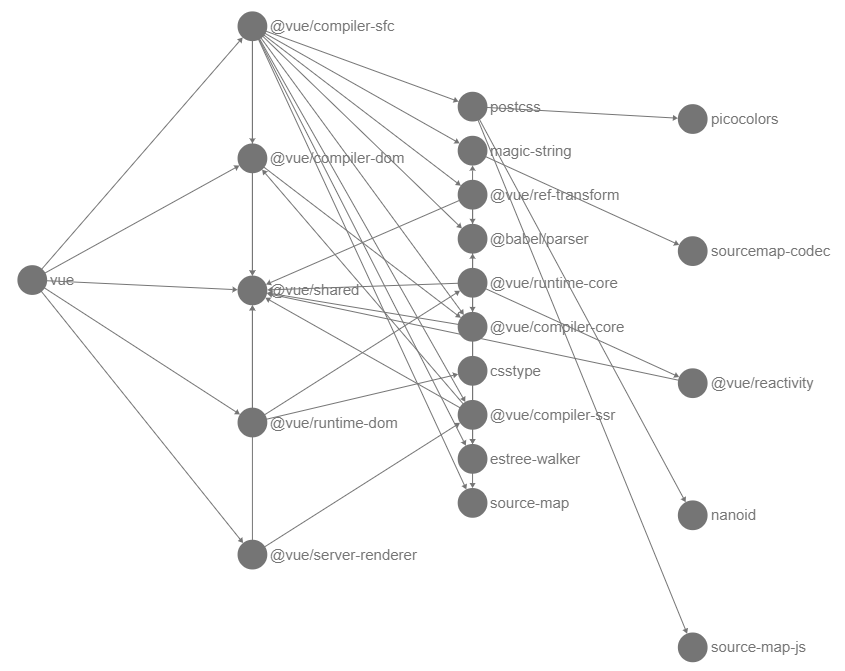
\includegraphics[scale=0.4]{images/graph_wrong.png}
	\caption{Rossz gráf elrendezés}
	\label{fig:graph_wrong}
\end{figure}

\pagebreak

\subsection{Gráfrendező Algoritmus}
Mint látható a \ref{fig:graph_wrong} ábrán, a gráf nem valósítja meg a DAG elrendezést. A gráf helyes elrendezését megvalósító, már létező algoritmust nem találtam, a legtöbb esetben az \textbf{npmgraph.an} példájához hasonlóan, randomizáltan, inkább hálós gráfot hoznak létre. \\

Ennek megfelelően saját algoritmust írtam a gráf csomópontjainak helyes elrendezésére. Az algoritmus két szakaszból épül fel, az 1. szakaszban (X koordináta) a horizontális rendezés történik a különböző szintekre, majd a 2. szakaszban (Y koordináta) az adott szinteken történik egy vertikális rendezés. 

\subsubsection{Gráfrendező Algoritmus: 1. Szakasz}

\begin{algorithm}
	\caption{Node X Coordinates}
	\centering
	\begin{algorithmic}
		\Require $nodes$ and $edges$		
		\State $changes \gets true$
		\While{ $changes$ }
			\State $changes \gets false$
			\ForAll{$edges$}
				\State Initialize $source$ and $target$
				\ForAll{$nodes$}
					\If{$edge.source = node$}
						\State $source \gets node$
					\ElsIf{$edge.target = node$}
						\State $target \gets node$
					\EndIf
					\If{$source$ is defined \textbf{and} $target$ is defined}
						\If{$source.x = target.x$}
							\State $target.x \gets target.x+1$
							\State $changes \gets true$
						\ElsIf{$source.x > target.x$}
							\State $target.x \gets source.x+1$
							\State $changes \gets true$
						\EndIf
						\State Break 
					\EndIf
				\EndFor
			\EndFor
		\EndWhile 
	\end{algorithmic}
\end{algorithm}

\pagebreak

\subsubsection{Gráfrendező Algoritmus: 2. Szakasz}

\begin{algorithm}
	\caption{Node Y Coordinates}
	\begin{algorithmic}	
		\Require $nodes$
		\State Initialize $nArray$
		\For{$i \gets 0$ \textbf{to} $nodes.length$}
			\If{$i < nodes.length$ \textbf{and} $nodes[i].x = nodes[i+1].x$}
				\State $nArray \gets nArray + nodes[i]$
			\ElsIf{$nArray.length > 0$}
				\State $nArray \gets nArray + nodes[i]$
				\State Initialize $offset$
				\If{$nArray[0]$ is even}
					\State $offset \gets 2/nArray.length$
				\Else
					\State $offset \gets 3/nArray.length$
				\EndIf
				\For{$j \gets 0$ \textbf{to} $nArray.length$}
					\If{$j = 0$}
						\State $nArray[j].y \gets Random(-0.5;\ 0.5)$
					\Else
						\If{$j$ is even}
						\State $nArray[j].y \gets nArray[j-2].y+offset$
						\Else
						\If{$j=1$}
						\State $nArray[j].y \gets nArray[j-1].y-offset$
						\Else
						\State $nArray[j].y \gets nArray[j-2].y-offset$
						\EndIf
						\EndIf
					\EndIf
				\EndFor
				\State $nArray.length \gets 0$
			\EndIf
		\EndFor
	\end{algorithmic}
\end{algorithm}

\pagebreak

\noindent\textbf{Az algoritmust lefutását követően Vue.JS \ref{fig:graph_wrong} ábrán látható felépítését az alábbi módon változtatta meg:}

\begin{figure}[!h]
	\centering
	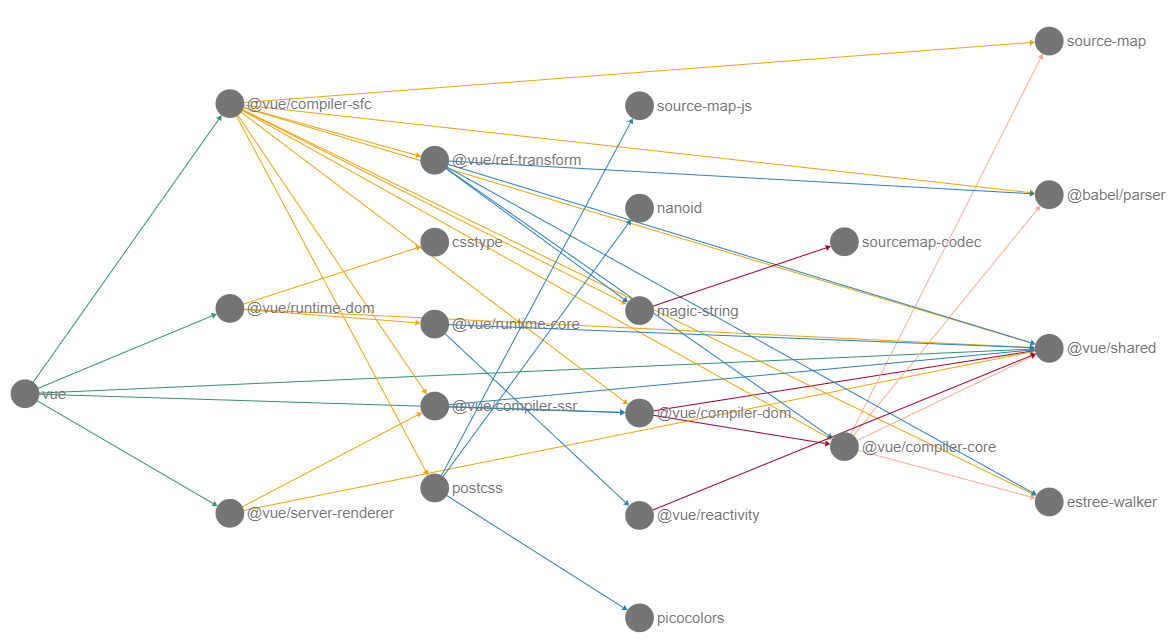
\includegraphics[scale=0.4]{images/graph_right.png}
	\caption{Helyes gráf elrendezés}
	\label{fig:graph_right}
\end{figure}

\noindent\textbf{Egy nem várt meglepetés:}\\

A tesztelés során akadtak olyan csomagok, ahol a gráf algoritmusa végtelen iterációban futott, ezzel lefagyasztva a programot.
Ennek az oka az volt, hogy egyes csomagok függőségei között olyan csomagverziók is voltak, amelyekben függőségként a gyökércsomag volt megjelölve, vagy esetleg kört eredményeztek a függőségi gráfban, ritkán egy szülő<-->gyermek kölcsönönös függési viszony alakult ki két csomag között. Ezek problémásak lehetnek, mivel elvben egy függőségi gráfban ilyennek nem szabadna előfordulni.

Az ilyen problémák kiszűrésére az algoritmus kapott egy olyan kiegészítést, hogy a gyökércsomag koordinátáit semmiképpen ne lehessen változtatni, illetve ha két iteráció között sem sikerül érdemben javítani az elrendezésen, kilép az algoritmus, mert nem tud tovább rendezni.\\

\subsubsection{Visszatérés}

A calculateGraph() attól függően, hogy szükséges-e, megrajzolja a gráfot, és visszatér a helyes csomópontokkal és élekkel feltöltött tömbbel a \textbf{graphDependencies()} függvénybe, ahol az adatokból létre fog hozni egy gráf objektumot, a gráf osztály példányosításával:

\begin{js}
let currentGraph = new Graph(graphEntities[0], graphEntities[1]);
\end{js}

\pagebreak

\subsection{Gráf Osztály}

\begin{js}
class Graph{
	constructor(nodes, edges){
		this.name = nodes[0].id;
		this.nodes = nodes;
		this.edges = edges;
	}
	getMaxDepth(){
	}
	getLinksPerDepth(){
	}
	getNodeDegrees(){
	}	
}
\end{js}

Ez az osztály tartalmaz minden olyan adattagot és metódust, amelyre a függőségi gráf elemzésénél szükség lesz. Vissza fogja adni a fokszámot, a gráf mélységét, és azt is, hogy mélységi szintenként hány függőség van.

\subsection{Gráf Elemzése}

Egy csomagot vizsgáló mód esetén az utolsó előtti lépés a függőségi gráf elemzése, amelynek könnyítésére jött létre a gráf osztály, amellyel egyszerűen tudjuk elemezni a gráfot. Az elemzések eredményeit grafikus módon a \textbf{chart.js} diagram készítő csomaggal fogja majd ábrázolni a program.

\subsubsection{Chart.js csomag}

A Chart.js egy egyszerű, könnyűsúlyú JavaScript csomag interaktív hisztogramok, diagramok létrehozására, ábrázolására.\\

A programban ezt a csomagot a \textbf{makeHistogram.js} fájl fogja implementálni, amelyben található egy makeHistogram() függvény. A funkció a következő adatokat fogja elvárni paraméterként: 

\begin{itemize}
	\item \texttt{"id"}: A HTML Div elem ID-ja, amelyet canvasként fog használni a hisztogram számára.
	\item \texttt{"dataArray"}: Az ábrázolandó y adatokat tartalmazó tömb.
	\item \texttt{"label"}: A hisztogram elnevezése.
	\item \texttt{"labArray"}: Az x tengely beosztásait tartalmazó tömb.
\end{itemize} 

A setHistogram() függvényt az analyseGraph() fogja meghívni, amely előkészíti azokat a HTML elemeket, amik szükségesek lesznek az elemzés eredményeinek megjelenítésére. A különböző eredményeket szövegesen vagy hisztogram formájában fogja megjeleníteni a Sidebar-on. Miután elvégezte az elemzéseket meghívja a setHistogram() funkciót, amely az adatokat a megjelenítő által elvárt formára hozza és meghívja a makeHistogram() függvényt, ami pedig kirajzolja a megfelelő reprezentatív hisztogramokat. 

\pagebreak
 
\noindent\textbf{Chart.js szintaktikája:}
 
\begin{js}
function makeHistogram(id, dataArray, label, labArray){
	const ctx = document.getElementById(id).getContext('2d');
	const chart = new Chart(ctx, {
		type: 'line',
		data: {
			labels: labArray,
			datasets: [{
				label: label,
				data: dataArray,
			}]
		},
		options: {
			scales: {
				xAxes: [{
				}],
				yAxes: [{
				}]
			}
		}
	});
}	
\end{js}

\subsection{Javaslattétel}

A csomag függőségeinek lekérdezésénél említésre került a kulcsszavak lekérdezése, ennek az oka a javaslattételhez kapcsolódik. Az eredeti megoldás egy külön lekérdezés volt minden csomag esetében, majd a válaszból kinyerésre kerültek a kulcsszavak. 

Mivel a függőségek esetében küldött kérésre kapott válaszban szintén szerepeltek a kulcsszavak a terhelés csökkentése és a futásidő javítása érdekében ott történik a kulcsszavak kinyerése és eltárolása is.

A megszerzett csomagok adatait tartalmazó objektumok így a kulcsszavakat is tárolni fogják.\\

A kulcsszavak elemzését az analyseGraph() függvény által meghívott \textbf{checkKeywords()} függvény fogja végezni, amely paraméterként bekéri az összegyűjtött csomagokat és függőségeket.

A csomagokat összehasonlítja és amennyiben nincsenek egymással függési viszonyban, illetve több a funkcionalitásukat leíró kulcsszavak több mint 50\%-os átfedésben vannak, esetleges redundanciaként kezeli.
Az ilyen csomagpárokat visszaadja egy tömbbe rendezve, melynek minden eleme tartalmazza a csomagok nevét, azok szüleit, és az átfedés mértékét \%-ban megadva.

Az analyseGraph() végül ezeket ki fogja írni a Sidebar aljára, mint esetleges redundáns funkcionalitású csomagokat.

A csomagok vizsgálata a fejlesztő feladata, a program funkcionalitása csak a kulcsszavak alapján tesz javaslatot, amely nem jelenti, hogy redundáns a csomagok funkcionalitása, viszont a kulcsszavak egyezése miatt lehetséges. 

\section{Függőségi Gráfok Statisztikai Vizsgálata}

Ebben a szekcióban a program másik felhasználási módja kerül bemutatásra, amely több csomag függőségi gráfjainak statisztikai elemzését teszi lehetővé.
Ezen mód alapjait nagyrészt lefedi az egy csomagos módnál bemutatott funkcionalitás, néhány kiegészítéssel. Az ismertetés során így a már áttekintet funkciókra csak hivatkozás fog történni.\\
 
A későbbiekben az első 1000 leggyakrabban használt csomagot és azok függőségeit fogjuk tekinteni a reprezentatív módon leszűkített teljes npm Registrynek, mivel a teljes Registry túl nagy lenne az elemzésre, bár a lehetőség elvben meg lenne rá.\\

A program több csomagos módra váltását követően meg lehet adni, hogy hány csomag függőségi gráfjának elemzését szeretnénk kérni, és hogy ezeket milyen paraméter alapján állítsa sorrendben és adja vissza a program. Az elemzést minimum egy csomagra lehet elindítani és az alapértelmezett rangsorolás a leggyakrabban használt csomagok szerint történik.\\

Ezt követően meghívásra kerül a handleSideBarEvents() modulból a \textbf{createStatistics.js} modul createStats() függvénye. Paraméterként a csomagok mennyiségét és a rangsorolási módot fogja kérni.

\subsubsection{Eltérések az egycsomagos módhoz képest:}

\begin{itemize}
	\item \textbf{searchPackages()} funkció
	\item \textbf{getGitData()} funkció
	\item A létrehozott függőségi gráfoknak csak felhasználja a szerkezetét, nem rajzolja ki
	\item Nem fogja az önálló gráfelemzéseket elvégezni
\end{itemize}

\subsection{searchPackages Modul}

A searchPackages modul a csomagok sorrendbe rendezett lekérésére alkalmas. A modul implementálja a Libraries.io API-ját, amely lehetővé teszi a csomagkezelő által nyilvántartott csomagok különböző elvek szerint rendezett lekérdezését. Az alapértelmezés a már említett leggyakrabban használt csomagok elve, azonban lehetőség van még SourceRank, csillagok száma, legfrissebb kiadású csomagok, függő csomagok száma, közreműködők száma és legújabb csomagok szerinti rendezésre is.\\

Az API működése paraméterezett kérésekkel történik, a Libraries.io search végpontja felé. Ezekre válaszul csomagokat tartalmazó JSON objektumokat ad vissza. A rangsorolt csomagokat oldalanként tárolja és adja vissza, amelynek a mérete maximum 100 elemű lehet. Ennek megfelelően egy 1000 csomagos lekérdezés esetén 10 x 100 csomag lekérdezése fog megtörténni, majd ezeket egy tömbként adja vissza a funkció. A kérések a már ismert fetchData() funkcióval történnek.

\subsubsection{Szükséges paraméterek:}
\begin{js}
	let params = {
		sort:sortBy, 
		per_page:size,
		page:1,
		platforms:"NPM",
		api_key:"576acbf22232eac6a3a6b05be774eecb"
	}
\end{js}

\subsubsection{Visszatérés és Megjelenítés}

A visszakapott csomagok függőségi gráfjait a createStats() függvény egyesével lekérdezi, az egy csomagos mód esetében tisztázott lépéssorozat segítségével, majd a visszakapott \textbf{Graph} objektumokat eltárolja egy tömbben.\\

A gráf objektumokat tartalmazó tömb adatait a megjelenítő hisztogramok típusának megfelelő formába rendezése után, a függések száma szerint csökkenő sorrendben a korábban már szintén tisztázott setHistogram() és makeHistogram() függvények segítségével az oldal "Canvas" részén jeleníti meg. Erre azért van szükség, mivel nagy mennyiségű csomagok esetén, itt lehetséges reprezentatív méretű hisztogramokat kirajzolni.

\subsection{Fájlszintű Elemzés} 
A csomagok statisztikai vizsgálatának egy igen fontos lépése a jegyzék szintű elemzése az adott csomagnak. Az elemzés során ki fog derülni:
\begin{itemize}
	\item A csomag mérete
	\item A csomag fájljainak száma
	\item A JavaScript fájlok aránya
	\item A TypeScript fájlok aránya
\end{itemize}

\subsubsection{Probléma}
Az elemzés módjának kivitelezésére a terv egy lokális vizsgálat volt, amely a következő okok miatt nem igazán bizonyult kivitelezhetőnek:
\begin{itemize}
	\item Minden vizsgálandó csomagnak lokálisan jelen kell lennie a rendszeren, amely nagy mennyiségű npm csomag letöltését eredményezné.
	\item A letöltéshez gyermek processz-re van szükség, hogy a JavaScript kódból futtatható legyen a telepítés.
	\item A lokális fájlok vizsgálatához a NodeJS filesystem API-ja szükséges.
	\item Mind a gyermek processz és filesystem kliens oldali használata biztonságtechnikai okokból korlátozásra került.
\end{itemize}

\subsubsection{Megoldás}
A kivitelezés megvalósítására a GitHub API-ja nyújtott lehetőséget, amely tanulmányozásának eredményeként kiderül, hogy képes a program által igényelt adatok szolgáltatására.\\

A program alapvetően két végpont URL címével dolgozik, melyek felé kéréseket intéz a megfelelő "tulajdonos/repo-név", illetve "branch" megadásával.
\begin{itemize}
	\item https://api.github.com/repos/\{repo\}
	\item https://api.github.com/repos/\{repo\}/git/trees/\{branch\}?recursive=1
\end{itemize}

Az első végpont a repository adatait adja vissza, majd ebből kinyerve az alapértelmezett branchet intéz kérést a program a második végpont felé, amely rekurzívan megkeresi és visszaadja a repository jegyzék struktúráját.

\subsubsection{Implementáció}
Minden csomag esetében két kérés történik a GitHub api felé, az első az általános adatok lekéréséhez, a második a jegyzék struktúra lekérdezéséhez.\\

A kéréseket a \textbf{getGitData()} függvény fogja elvégezni, majd a választ a megfelelő formában visszaadni.

\begin{js}
	function getGitData(repo, urlType, branch=""){  
		*do stuff*
		return pkg;
	}
\end{js}
Paraméterként a repository tulajdonosát és nevét kéri be "owner/name" formában, az URL típusát, hogy általános vagy jegyzék lekérdezéshez állítsa be az URL-t, illetve jegyzékek esetén a "branch" nevét.\\

A getGitData() a már ismert fetchData() függvényt fogja alkalmazni a kérésekhez.

\subsubsection{Fetch Korlátozások}
Az adatok megszerzéséhez szükséges kérések számát a GitHub API limitálja. Alapértelmezetten ez 60 kérés óránként, ami igen kevés, maximum 30 csomag elemzésére elég egy órában.

Azonban, ha authorizált felhasználó intézi a kéréseket akkor ez a szám 5000 kérésre emelkedik óránként, ami már bőven elég az 1000 csomagos vizsgálathoz.\\

A GitHub minden felhasználó számára biztosítja az Auth Tokeneket, amit a kérés Headerjébe helyezve lehet használni. Egy Auth Token igénylésénél meg lehet adni milyen privilégiumokkal rendelkezzen. A programban használt Token semmilyen privilégiummal nem rendelkezik, pusztán jelzi, hogy a lekérdezés felhasználó által történik.\\

A fetchData.js modul így kiegészítésre került a GitHub Token használatával.

\pagebreak

\begin{js}
function fetchData(url, token=false){
	let headers = {"Content-Type": "application/json"};
	
	if(token){
		headers["Authorization"] = "token "+getToken();
	}
	
	let response = await fetch(url, {headers,});
	
	if (!response.ok) {
		throw new Error(response.status);
	}
	
	return response.json();
}

function getToken(){
	const decipher = crypto.createDecipheriv();
	const decrypted = Buffer.concat([decipher.update(Buffer.from()),
						decipher.final()]);
	
	return decrypted.toString();
}
\end{js}
\textbf{Token Probléma:} A kód GitHubra commitolása során a rendszer észrevette a kódban megadott Token jellegű adatot, így visszavonta a Tokent. 

Ezért szükség volt a Token titkosítására, majd az így titkosított Token került megadásra a kódban és csak futásidőben fog visszafejtésre kerülni, így a GitHub számára nem Token jellegű a karaktersorozat és nem vonja vissza.

A Token egyébként nem okoz biztonsági problémát, mivel már említésre került, hogy a Tokenhez nincs semmilyen privilégium társítva, pusztán arra alkalmas, hogy a kéréseknél jelezzük, hogy authorizált kérésről van szó.\\

A getGitData() adatait a \textbf{analyseSource()} függvény fogja felhasználni, amely csomagonként az alábbi információt fogja szolgáltatni a createStats() függvény számára:

\begin{js}
	{Package:, Size:, Files:, JS_Files:, TS_Files:}
\end{js}
Azaz csomagnév, csomagméret MB-ban, fájlok száma, JavaScript fájlok aránya \%-ban megadva, TypeScript fájlok aránya \%-ban megadva.

\subsubsection{Visszatérés}

A fent leírt objektumok tömbjével fog visszatérni a createStats() függvényben, amelyet felhasználva az a setHistogram() és makeHistogram() fügvényekkel ábrázolni fog a függőségek száma szerint csökkenő sorrendben.

